\documentclass[border=10pt]{standalone}
\usepackage{tikz}
\usepackage{tikz}
\usepackage{circuitikz}
\usetikzlibrary{arrows,positioning,shapes.geometric}
\begin{document}
\begin{normalsize}
 \tikzset{every picture/.style={line width=0.75pt}} %set default line width to 0.75pt        

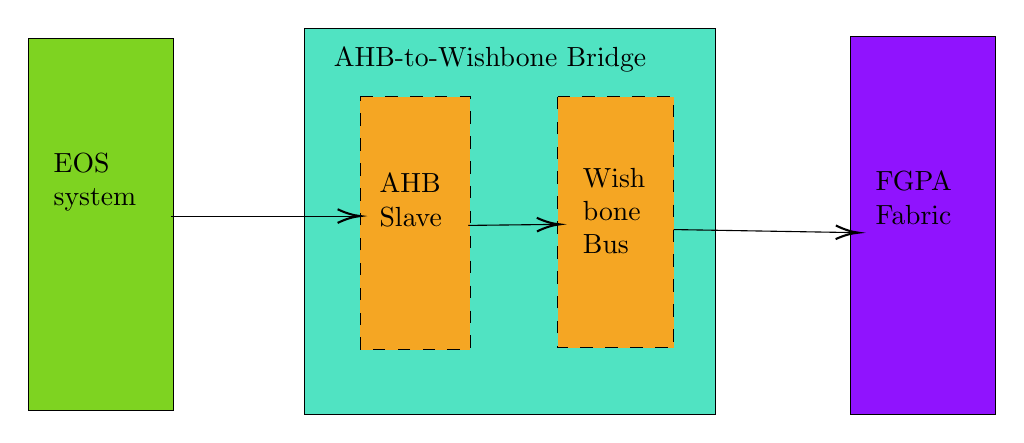
\begin{tikzpicture}[x=0.75pt,y=0.75pt,yscale=-1,xscale=1]
%uncomment if require: \path (0,391); %set diagram left start at 0, and has height of 391

%Shape: Rectangle [id:dp9464347346403436] 
\draw  [fill={rgb, 255:red, 126; green, 211; blue, 33 }  ,fill opacity=1 ] (34,96) -- (104,96) -- (104,275) -- (34,275) -- cycle ;
%Shape: Rectangle [id:dp5425045207301228] 
\draw  [fill={rgb, 255:red, 80; green, 227; blue, 194 }  ,fill opacity=1 ] (167,91) -- (365,91) -- (365,277) -- (167,277) -- cycle ;
%Shape: Rectangle [id:dp0010939187451719512] 
\draw  [fill={rgb, 255:red, 245; green, 166; blue, 35 }  ,fill opacity=1 ][dash pattern={on 4.5pt off 4.5pt}] (194,124) -- (247,124) -- (247,246) -- (194,246) -- cycle ;
%Shape: Rectangle [id:dp10703956518255331] 
\draw  [fill={rgb, 255:red, 245; green, 166; blue, 35 }  ,fill opacity=1 ][dash pattern={on 4.5pt off 4.5pt}] (289,124) -- (345,124) -- (345,245) -- (289,245) -- cycle ;
%Shape: Rectangle [id:dp3967502906935467] 
\draw  [fill={rgb, 255:red, 144; green, 19; blue, 254 }  ,fill opacity=1 ] (430,95) -- (500,95) -- (500,277) -- (430,277) -- cycle ;
%Straight Lines [id:da9811686598138952] 
\draw    (103,181.5) -- (192,181.5) ;
\draw [shift={(194,181.5)}, rotate = 180] [color={rgb, 255:red, 0; green, 0; blue, 0 }  ][line width=0.75]    (10.93,-3.29) .. controls (6.95,-1.4) and (3.31,-0.3) .. (0,0) .. controls (3.31,0.3) and (6.95,1.4) .. (10.93,3.29)   ;
%Straight Lines [id:da7120879916913804] 
\draw    (246,186) -- (288,185.52) ;
\draw [shift={(290,185.5)}, rotate = 179.35] [color={rgb, 255:red, 0; green, 0; blue, 0 }  ][line width=0.75]    (10.93,-3.29) .. controls (6.95,-1.4) and (3.31,-0.3) .. (0,0) .. controls (3.31,0.3) and (6.95,1.4) .. (10.93,3.29)   ;
%Straight Lines [id:da18993536842155556] 
\draw    (345,188) -- (432,189.47) ;
\draw [shift={(434,189.5)}, rotate = 180.97] [color={rgb, 255:red, 0; green, 0; blue, 0 }  ][line width=0.75]    (10.93,-3.29) .. controls (6.95,-1.4) and (3.31,-0.3) .. (0,0) .. controls (3.31,0.3) and (6.95,1.4) .. (10.93,3.29)   ;

% Text Node
\draw (45,150) node [anchor=north west][inner sep=0.75pt]   [align=left] { EOS\\system};
% Text Node
\draw (202,160) node [anchor=north west][inner sep=0.75pt]   [align=left] {AHB\\Slave};
% Text Node
\draw (300,157) node [anchor=north west][inner sep=0.75pt]   [align=left] {Wish\\bone \\Bus };
% Text Node
\draw (441,159) node [anchor=north west][inner sep=0.75pt]   [align=left] {FGPA\\Fabric};
% Text Node
\draw (180,99) node [anchor=north west][inner sep=0.75pt]   [align=left] {AHB-to-Wishbone Bridge};


\end{tikzpicture}
\end{normalsize}
\end{document}
